% !TEX root = ../main.tex
\paragraph{Back Angle Neutron Detector (BAND)}
    \begin{wrapfigure}{r}{0.49\textwidth}
        \centering\frame{
        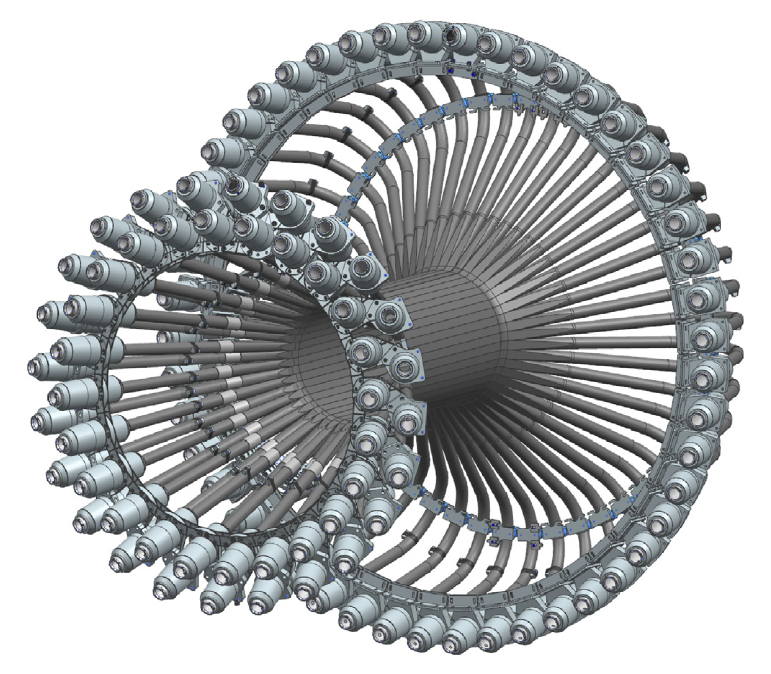
\includegraphics[width=\linewidth]{11experiment/img/22ctof.png}}
        \caption[Central Time-of-Flight]{Render of the Central Time-of-Flight.
        The render shows CTOF's 48 scintillator bars outfitted with light guides, PMTs, and magnetic shields at both ends of each counter.}
        \label{fig::ctof}
    \end{wrapfigure}

    The CLAS12 spectrometer includes the BAND as a dedicated detector for neutron detection at backward angles.
    Positioned 3 metres upstream of the target, the BAND is designed to detect backward-scattered neutrons with momenta ranging from 0.25 to 0.7 GeV.

    The BAND detector consists of 18 horizontal rows and five layers of scintillator bars.
    Each scintillator bar is equipped with PMT readout on both ends to measure the TOF of neutrons originating from the target.
    Additionally, there is an extra 1 cm scintillation layer specifically designed to veto charged particles, ensuring that only neutrons are detected.

    Covering a polar angle range from $155\degree$ to $175\degree$, the BAND detector achieves a design neutron detection efficiency of $35\%$.
    It also provides a momentum resolution of approximately $1.5\%$, allowing for precise measurements of the momentum of the detected neutrons \cite{segarra2020}.

    By utilizing the BAND detector, the CLAS12 spectrometer is capable of detecting and characterizing backward-scattered neutrons, providing valuable information for various physics studies and experiments conducted at CLAS12.
